\documentclass[12pt]{article}
\usepackage{hyperref}
\usepackage{listings}
\usepackage[margin=1in]{geometry}
\usepackage{enumitem}
\usepackage{multicol}
\usepackage{array}
\usepackage{titlesec}
\usepackage{helvet}
\renewcommand{\familydefault}{\sfdefault}
\usepackage{amsmath}     % For math equations
\usepackage{amssymb}     % For advanced math symbols
\usepackage{amsfonts} % For math fonts
\usepackage{gvv}
\usepackage{esint}
\usepackage[utf8]{inputenc}
\usepackage{graphicx}
\usepackage{pgfplots}
\pgfplotsset{compat=1.18}
\titleformat{\section}{\bfseries\large}{\thesection.}{1em}{}
\setlength{\parindent}{0pt}
\setlength{\parskip}{6pt}
\usepackage{multirow}
\usepackage{float}
\usepackage{caption}


\begin{document}

\textbf{Problem 12.214} 

The eigenvector pair of the matrix
\begin{align}
A = \myvec{3 & 4 \\ 4 & -3}
\end{align}
is (PI 2008)

\textbf{Options:}
\begin{align}
\text{(a)} \quad & \myvec{2 \\ 1}, \; \myvec{1 \\ -2} \\
\text{(b)} \quad & \myvec{1 \\ 2}, \; \myvec{2 \\ -1} \\
\text{(c)} \quad & \myvec{1 \\ -2}, \; \myvec{-2 \\ -1} \\
\text{(d)} \quad & \myvec{1 \\ -2}, \; \myvec{2 \\ 1}
\end{align}


\textbf{Input Variables:}

\begin{table}[H]
\centering
\begin{tabular}{|c|c|}
\hline
Symbol & Description \\
\hline
$A$ & Given matrix $\myvec{3 & 4 \\ 4 & -3}$ \\
$\lambda$ & Eigenvalue of $A$ \\
$\vec{v}$ & Corresponding eigenvector \\
\hline
\end{tabular}
\end{table}

\textbf{Solution:}

\begin{align}
A &= \myvec{3 & 4 \\ 4 & -3} \\[6pt]
\det(A - \lambda I) &= 
\det\myvec{3-\lambda & 4 \\ 4 & -3-\lambda} \\[6pt]
&= (3-\lambda)(-3-\lambda) - 16 \\[6pt]
&= \lambda^2 - 25 \\[6pt]
\Rightarrow \lambda &= \pm 5
\end{align}

\textbf{For $\lambda = 5$:}
\begin{align}
(A - 5I)\vec{v} &= 0 \\[6pt]
\myvec{-2 & 4 \\ 4 & -8}\myvec{x \\ y} &= \vec{0} \\[6pt]
-2x + 4y &= 0 \Rightarrow x = 2y \\[6pt]
\vec{v_1} &= \myvec{2 \\ 1}
\end{align}

\textbf{For $\lambda = -5$:}
\begin{align}
(A + 5I)\vec{v} &= 0 \\[6pt]
\myvec{8 & 4 \\ 4 & 2}\myvec{x \\ y} &= \vec{0} \\[6pt]
8x + 4y &= 0 \Rightarrow y = -2x \\[6pt]
\vec{v_2} &= \myvec{1 \\ -2}
\end{align}

\textbf{Hence, the correct eigenvector pair is}
\begin{align}
\vec{v_1} = \myvec{2 \\ 1}, \quad \vec{v_2} = \myvec{1 \\ -2}.
\end{align}

\textbf{Answer: (a)}

\begin{figure}[H]
    \centering
    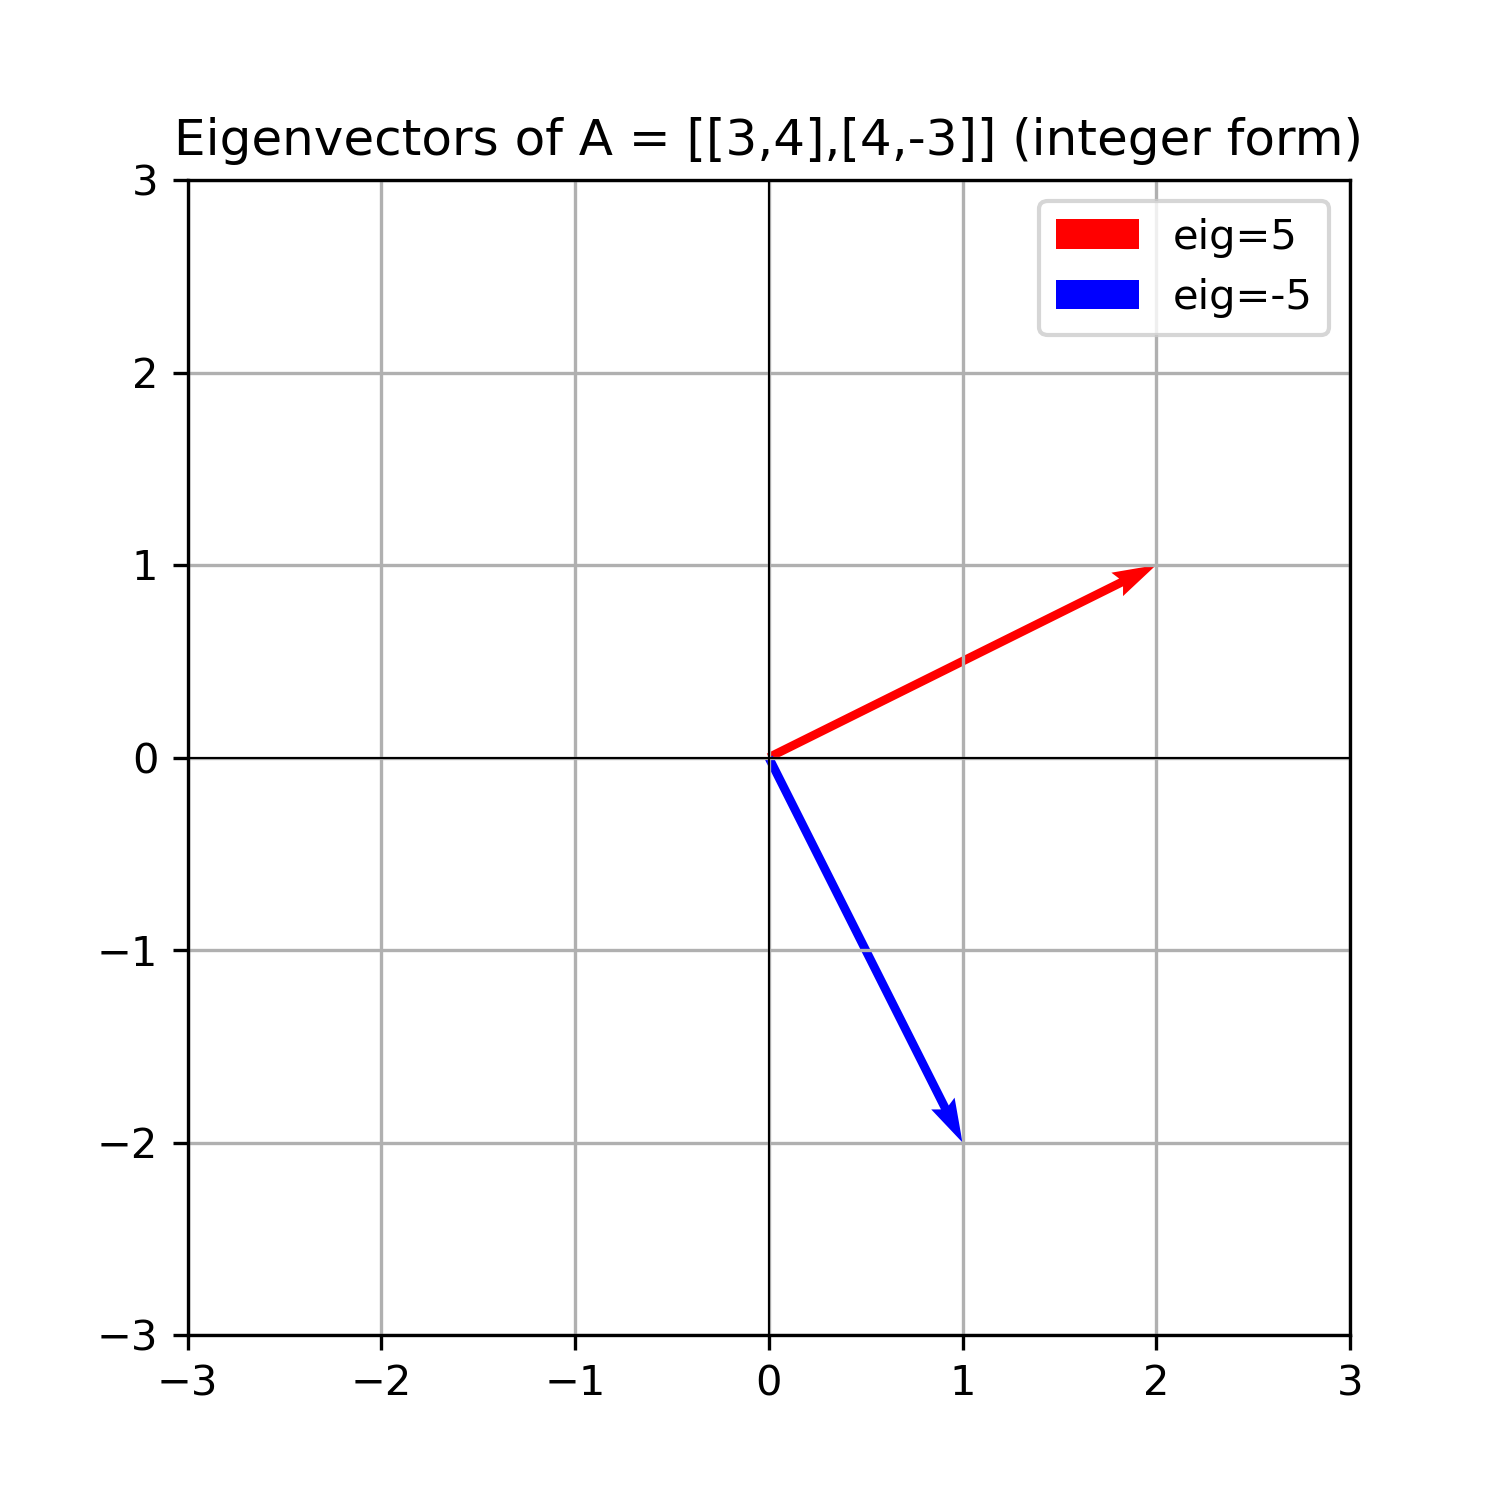
\includegraphics[width=0.9\columnwidth]{figs/eigenvectors_problem_adjusted.png}
    \caption{}
    \label{fig:placeholder}
\end{figure}


\end{document}
